% Current BCS model, "Attention Is All You Need" style (bottom-to-top flow).
% Left: region segmenter (fine-tuned DINOv2-B + FPN).
% Right: frozen DINOv2-L -> per-region average -> ridge -> BCS.
% Build: pdflatex model_bcs_vertical_en.tex
\documentclass[tikz,border=8pt]{standalone}
\usepackage[utf8]{inputenc}
\usepackage[T1]{fontenc}
\usetikzlibrary{arrows.meta,calc,backgrounds,fit}

\definecolor{attn}{HTML}{FCE0C4}
\definecolor{norm}{HTML}{F3F5C9}
\definecolor{ff}{HTML}{C9E7F5}
\definecolor{emb}{HTML}{FADADD}
\definecolor{dec}{HTML}{DCD3EE}
\definecolor{reg}{HTML}{D5EBD9}
\definecolor{bloque}{HTML}{F2F2F2}

\tikzset{
  font=\sffamily\small, >={Stealth[length=2mm]},
  capa/.style={draw, rounded corners=4pt, line width=0.6pt, minimum width=3.4cm,
               minimum height=0.62cm, align=center, fill=#1},
  alta/.style={capa=#1, minimum height=0.95cm},
  suma/.style={draw, circle, line width=0.6pt, inner sep=0pt, minimum size=0.42cm, fill=white},
  flecha/.style={->, line width=0.6pt},
  linea/.style={line width=0.6pt},
  marco/.style={draw, rounded corners=8pt, line width=0.6pt, fill=bloque},
}
\newcommand{\plus}[2]{\node[suma] (#1) at #2 {};
  \draw[line width=0.6pt] (#1.north) -- (#1.south) (#1.west) -- (#1.east);}

% Input + ViT encoder block centered at x=#1, name prefix #2
\newcommand{\vit}[2]{
  \node (#2in) at (#1,-0.3) {Image};
  \node[capa=emb] (#2pe) at (#1,0.8) {Patch embedding};
  \plus{#2pos}{(#1,1.85)}
  \node[anchor=east, font=\sffamily\scriptsize] (#2post) at (#1-0.55,1.85) {Position};
  \draw[flecha] (#2in) -- (#2pe); \draw[flecha] (#2pe) -- (#2pos); \draw[flecha] (#2post) -- (#2pos);
  \draw[linea] (#2pos.north) -- (#1,2.95);
  \node[capa=norm] (#2ln1) at (#1,3.55) {Layer Norm};
  \node[alta=attn] (#2mha) at (#1,4.85) {Multi-Head\\Attention};
  \plus{#2add1}{(#1,6.0)}
  \node[capa=norm] (#2ln2) at (#1,6.85) {Layer Norm};
  \node[alta=ff]   (#2mlp) at (#1,8.05) {MLP};
  \plus{#2add2}{(#1,9.2)}
  \draw[flecha] (#1,2.95) -- (#2ln1);
  \draw[linea] (#2ln1.north) -- ++(0,0.2) coordinate (#2qkv);
  \foreach \dx in {-0.8,0,0.8} \draw[flecha] (#2qkv) -| ($(#2mha.south)+(\dx,0)$);
  \draw[flecha] (#2mha) -- (#2add1); \draw[flecha] (#2add1) -- (#2ln2);
  \draw[flecha] (#2ln2) -- (#2mlp);  \draw[flecha] (#2mlp) -- (#2add2);
  \draw[flecha, rounded corners=3pt] (#1,3.05) -- ++(-2.15,0) |- (#2add1.west);
  \draw[flecha, rounded corners=3pt] (#1,6.42) -- ++(-2.15,0) |- (#2add2.west);
  \begin{scope}[on background layer]
    \node[marco, fit={(#1-2.35,2.8) (#1+1.95,9.6)}] (#2blk) {};
  \end{scope}
}

\begin{document}
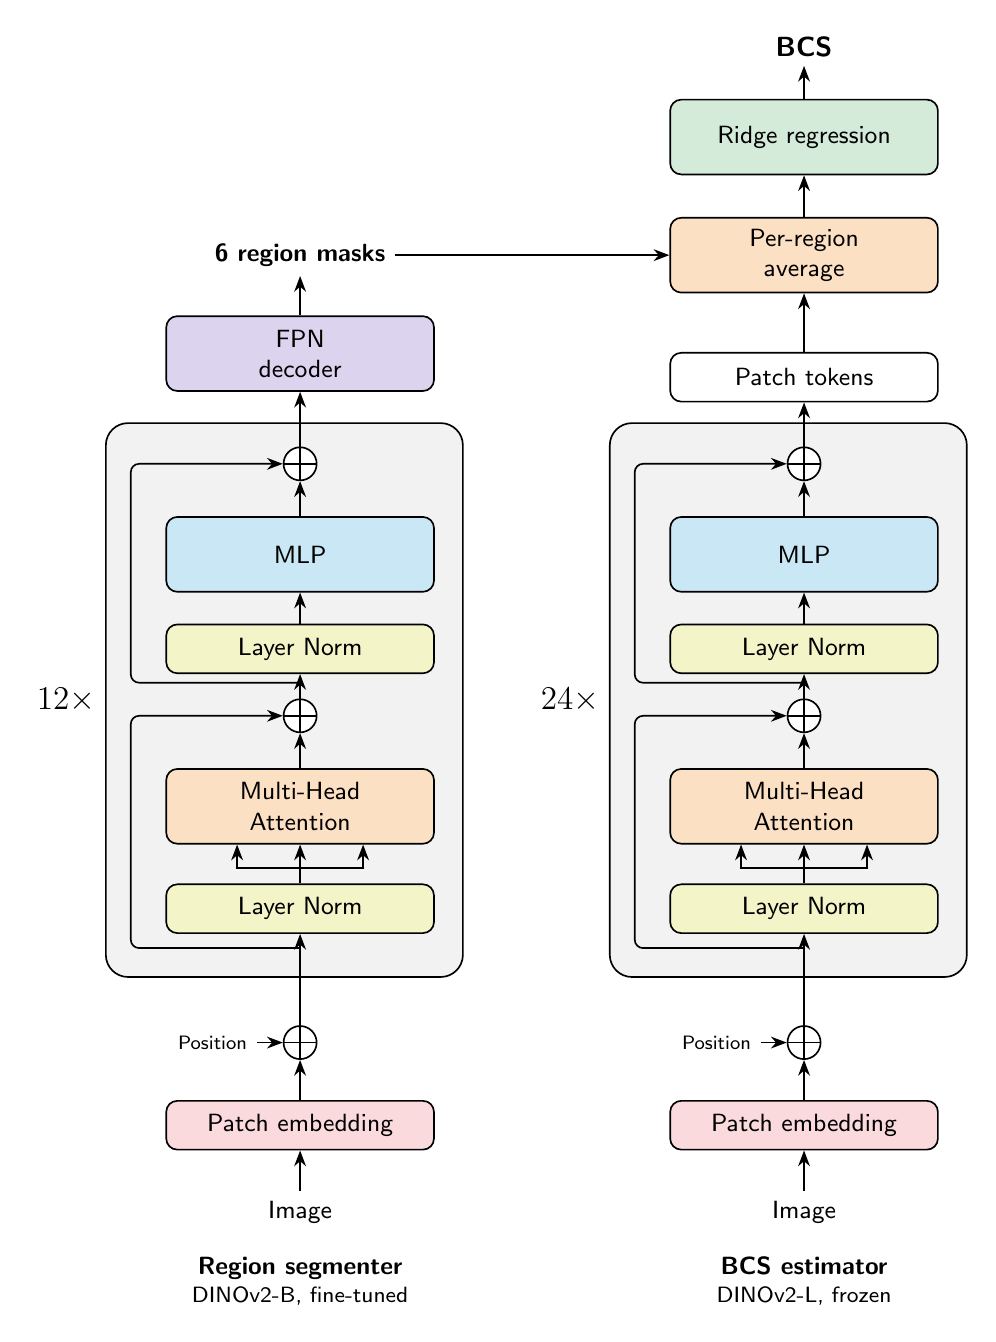
\begin{tikzpicture}

% ---------- Region segmenter ----------
\vit{0}{A}
\node[font=\sffamily\large, anchor=east] at (Ablk.west) {$12\times$};
\node[alta=dec] (fpn) at (0,10.6)  {FPN\\decoder};
\node (masks)         at (0,11.85) {\textbf{6 region masks}};
\draw[flecha] (Aadd2) -- (fpn); \draw[flecha] (fpn) -- (masks);
\node[font=\sffamily\small\bfseries, align=center, anchor=north] at (0,-0.75) {Region segmenter\\[-1pt]\mdseries\footnotesize DINOv2-B, fine-tuned};

% ---------- BCS estimator ----------
\def\xb{6.4}
\vit{\xb}{B}
\node[font=\sffamily\large, anchor=east] at (Bblk.west) {$24\times$};
\node[capa=white] (tok)   at (\xb,10.3)  {Patch tokens};
\node[alta=attn]  (pool)  at (\xb,11.85) {Per-region\\average};
\node[alta=reg]   (ridge) at (\xb,13.35) {Ridge regression};
\node[font=\sffamily\bfseries] (bcs) at (\xb,14.5) {BCS};
\draw[flecha] (Badd2) -- (tok); \draw[flecha] (tok) -- (pool);
\draw[flecha] (pool) -- (ridge); \draw[flecha] (ridge) -- (bcs);
\draw[flecha] (masks) -- (pool);
\node[font=\sffamily\small\bfseries, align=center, anchor=north] at (\xb,-0.75) {BCS estimator\\[-1pt]\mdseries\footnotesize DINOv2-L, frozen};

\end{tikzpicture}
\end{document}
